\documentclass[ProjectDLO]{subfiles}
% WARNING: AuCTeX local variables only get reset when file is loaded
% and differ between this file and BufferStockTheory.tex
% so must re-load whichever file you want to compile with C-x C-v

% WARNING: Different AucTeX execution depending on whether
% 0. Being compiled as standalone document
%    * Compile main once
%    * Then compile this one
%    * Keep compiling until nothing changes
% 0. Being compiled as subfile of main document
%    * Just compile main document repeatedly

\input{./econtexRoot}
\input{\LaTeXInputs/econtex_onlyinsubfile}
\onlyinsubfile{\externaldocument{ProjectDLO}} % Get xrefs -- esp to appendix -- from main file; only works properly if main file has already been compiled;

\begin{document}

% Attempted to make all lines used for Web version contain {Web} (or version with only single curly brace at end) so can be removed with sed
\providecommand{\versn}{pdf} % Version; like, web or pdf or journal submission
\ifthenelse{\boolean{Web}}{    % {Web}
  \renewcommand{\versn}{Web}     % Too hard to figure out passing -output-directory through make4ht through htlatex, so web version is compiled with junk files in main directory
  \renewcommand{\rootFromOut}{.} % {Web}
}{}  % {Web}

% Tiny info header at top to track git commit
%\hfill{\tiny \jobname~\versn~\today~{at} \DTMcurrenttime, \input{\ResourcesDir/.git-source-commit}~~\input{\ResourcesDir/.git-public-commit}}

\title{Price Rigidities \\ An attempt at a new angle}

\author{David L. Osten\authNum}

\keywords{Wage Price Pass Through, Wage Price Spiral, Labor Productivity, Wage Productivity Gap, Spatial Wage Differences, Spatial Price Differences}

%\jelclass{D81, D91, E21 \par
%  \href{https://econ-ark.org}{\includegraphics{\ResourcesDir/PoweredByEconARK}}
%}

\renewcommand{\forcedate}{December 21, 2021}\date{\forcedate}

\maketitle
\hypertarget{abstract}{This paper tries to bridge the recent findings of a weakening of pass through from wages to prices, especially in manufacturing, to the structual changes in the labor market since 1985}
\begin{abstract}

\end{abstract}


% Various resources
\hypertarget{links}{}

%\begin{footnotesize}
%  \parbox{0.9\textwidth}{
%    \begin{center}
%      \begin{tabbing}
%          \texttt{Dashboard:~} \= \= \texttt{\url{https://econ-ark.org/materials/BufferStockTheory?dashboard}} \\
%          \texttt{~~~REMARK:~} \> \> \texttt{\url{https://econ-ark.org/materials/BufferStockTheory}} \\ % Owner is defined in Resources/owner.tex
%          \texttt{~~~~~html:~} \> \> \texttt{\href{https://\owner.github.io/BufferStockTheory/}{https://\owner.github.io/BufferStockTheory/}} \\ % Owner is defined in Resources/owner.tex
%          \texttt{~~~~~~PDF:~} \> \> \texttt{\href{https://\owner.github.io/BufferStockTheory/BufferStockTheory.pdf}{https://\owner.github.io/BufferStockTheory/BufferStockTheory.pdf}} \\ % Owner is defined in% Resources/owner.tex
%          \texttt{~~~Slides:~} \> \> \texttt{\href{https://\owner.github.io/BufferStockTheory/BufferStockTheory-Slides.pdf}{https://\owner.github.io/BufferStockTheory/BufferStockTheory-Slides.pdf}} \\
%          \texttt{~Appendix:~} \> \> \texttt{\href{https://\owner.github.io/BufferStockTheory\#Appendices}{https://\owner.github.io/BufferStockTheory\#Appendices}}    \\
%          \texttt{~~~GitHub:~} \> \> \texttt{\href{https://github.com/\owner/BufferStockTheory}{https://github.com/\owner/BufferStockTheory}} \\
%      \end{tabbing}
%    \end{center}
%    The \href{https://econ-ark.org/materials/BufferStockTheory?dashboard}{dashboard} lets users see consequences of alternative parameters in an interactive framework.} % end parbox{\textwidth}
%\end{footnotesize}

\begin{authorsinfo}
  \name{Contact: \href{mailto:dosten1@jhu.edu}{\texttt{dosten1@jhu.edu}}, Department of Economics, 590 Wyman Hall, Johns Hopkins University, Baltimore, MD 21218.}
\end{authorsinfo}

\newcommand{\thankstext}{The paper benefitted substantially from helpful comments by Prof. C. Carroll, Prof. L. Ball and Prof. R. Moffitt from the Department of Economics of the Johns Hopkins University. Further, I would like to thank my fellow PhD students for their comments and critical questions.}

\ifthenelse{\boolean{Web}}{}{
  \begin{minipage}{0.9\textwidth}
    \tiny \thankstext
\end{minipage}
} % {Web}
{\titlepagefinish}



\section{The Introduction}


\hypertarget{Introduction}{}
%\section{Introduction}\label{sec:intro}
\newcommand{\introduction}{The wage price spiral has seen considerable attention in the 80s and 90s in the wake of the high inflation during the 60s and 70s. Since then the interest in the topic has followed the steady decline of the inflation rate. The recent contributions concentrated on explaining how the mechanism of the wage price spiral got muted over time and can therefore explain the surprisingly low inflation rates of the 2000s.\cite{Mehra2000} found that wages only had a significant effect on prices in the high inflation era of the 60s and 70s, but not in the 50s, 80s and 90s. It stands to reason that either lasting periods of high inflation are only observed if the wage price spiral is effctive, or that an elevated level of inflation is needed to start the spiral. This distinction is particularly interesting in light of the revived inflation rates in of the 2020s. The big question is, will this start sufficient upward pressure on wages to spin the spiral into action, or are there underlying forces that muted the pass through so that rising prices are not self-reinforcing.\\

Peneva and Rudd (2015) and more recently \cite{Heiseetal2020} found a weakened pass through from wages to prices, which \cite{Heiseetal2020} explain by import competition and increased market concentration in the manifacturing sector. \cite{Heiseetal2020} do control for total factor productivity (TFP) but not for labor productivity. In light of the structural changes since the mid 80s this might be a flaw in their analysis, as wages have been falling behind labor productivity between 1985 and 2012. Since then they have been stagnating and even slightly declining (see Figure 123). It might be worth exploring how much this wage-productivity gap influences manufacturers price setting decisions.} 

\begin{minipage}{0.9\textwidth}
    \introduction
\end{minipage}

\hypertarget{The-Model}{}

\section{The Model}

\subsection{Setup}\label{subsec:Setup}


\begin{verbatimwrite}{\EqDir/OLG}
  \begin{align}% \label{eq:OLG}
    \bar{k} = \left[\frac{(1-\epsilon)\beta}{\Xi (1+\beta)}^{1/(1-\epsilon)} \right]
  \end{align}
\end{verbatimwrite}
  \begin{align}% \label{eq:OLG}
    \bar{k} = \left[\frac{(1-\epsilon)\beta}{\Xi (1+\beta)}^{1/(1-\epsilon)} \right]
  \end{align}



%\providecommand{\figName}{RelatePFGICFHWCRICPFFVAC} % Allows generic definition of hypertargets based on title of figure
%\providecommand{\figFile}{\figName} %  and on filename
%\hypertarget{\figFile}{}
%\hypertarget{\figName}{}
%\input{\FigDir/\figName} % Read in the tex to generate the figure

\hypertarget{PF-Constrained-Solution}{}
\hypertarget{Constrained-Solution}{}

\newlength\TableWidth
\newsavebox{\Parameters}
\begin{table}
  \centering
\renewcommand{\arraystretch}{1.2}
  \caption{Microeconomic Model Calibration}\label{table:testable}
\sbox{\Parameters}{
\begin{tabular}{|c|ccl|c|}
\hline
\multicolumn{5}{|l|}{Calibrated Parameters}  \\ \hline
Test1                     & \multicolumn{1}{c}{Parameter} & Value & \multicolumn{2}{c|}{Source}\\ \hline
Test2  & \multicolumn{1}{c}{$\PGro$} & 1.03 & \multicolumn{2}{c|}{PSID: Carroll (1992)} \\
Test3                 & \multicolumn{1}{c}{$\Rfree$} & 1.04 & \multicolumn{2}{c|}{Conventional} \\
Test4          & \multicolumn{1}{c}{$\beta$} & 0.96 & \multicolumn{2}{c|}{Conventional} \\
Test5 & \multicolumn{1}{c}{$\CRRA$} & 2 & \multicolumn{2}{c|}{Conventional} \\
Test6      & \multicolumn{1}{c}{$\pZero$} & 0.005 & \multicolumn{2}{c|}{PSID: Carroll (1992)} \\
Test7  & \multicolumn{1}{c}{$\sigma_{\pshk}$} & 0.1 & \multicolumn{2}{c|}{PSID: Carroll (1992)} \\
Test8 & \multicolumn{1}{c}{$\sigma_{\theta}$} & 0.1 & \multicolumn{2}{c|}{PSID: Carroll (1992)} \\ \hline
\end{tabular}
} % End \sbox

\settowidth\TableWidth{\usebox{\Parameters}}
\usebox{\Parameters}
\end{table}



\begin{figure}[ht]
  \centerline{
    \includegraphics[width=3.5in]{\FigDir/StickyPriceLogic}
  }
  \caption{PF Unconstrained Model: Relation of \GICRaw, \FHWC, \RIC, and \PFFVAC} \label{fig:StickyPriceLogic}
  \footnotesize{A first visualization of the model's logic}
\end{figure}
 % Read in the tex to generate the figure

\hypertarget{DLOTestFig}{}
\begin{figure}[tbp]
\centerline{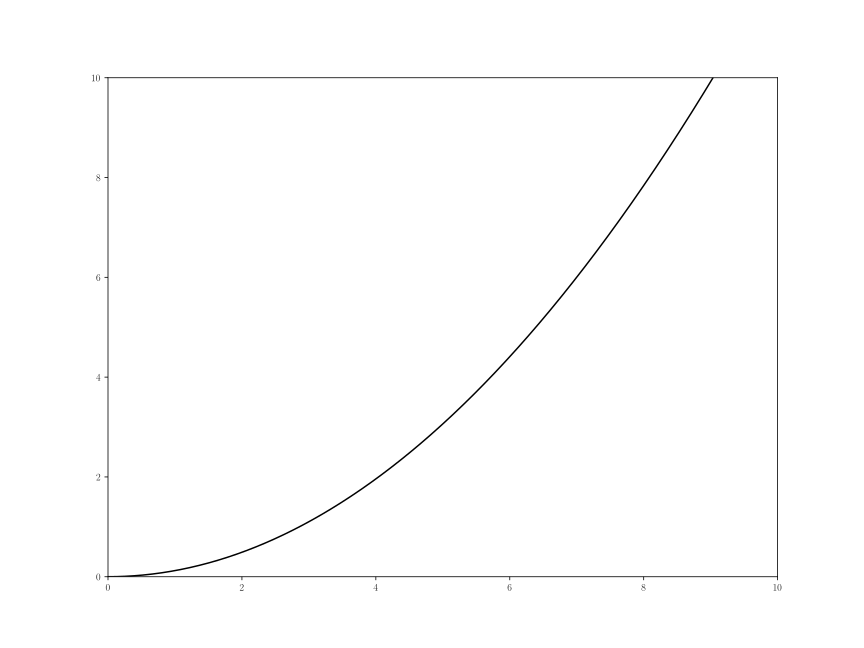
\includegraphics[width=6in]{\FigDir/DLOTestFig}}
\caption{Test Figure from Jupyter Notebook}
\label{fig:DLOTestFig}
\end{figure}


Just a citation test: \cite{DostenTest}





% %The paper's results are all easily reproducible \href{https://econ-ark.org/_materials/BufferStockTheory?launch}{interactively on the web} or \href{https://github.com/econ-ark/BufferStockTheory}{on any standard computer system}.  Such reproducibility reflects the paper's use of the open-source \href{https://econ-ark.org}{Econ-ARK} toolkit, which is used to generate all of the quantitative results of the paper, and which integrally incorporates all of the analytical insights of the paper.

% % The Dummy equation below sems to be needed to get the equation numbering in the appendix
% % reliably to start at the next number after the last actual equation number used in the paper

% \clearpage\vfill\eject
% \begin{equation*}
%   \label{eq:Dummy}
% \end{equation*}

% \onlyinsubfile{\bibliography{
%     \texname, % subfile inherits texname from preamble of parent
%     \econtexBib % Default bib database is in Resources/LaTeXInputs
%   }}

\onlyinsubfile{\input{\LaTeXInputs/bibliography_blend}}
%\bibliography{economics}
\end{document}
\endinput

% If you are editing in Emacs-AucTeX, modify the lines below for your system (otherwise ignore)
% Local Variables:
% eval: (setq TeX-command-list  (assq-delete-all (car (assoc "BibTeX" TeX-command-list)) TeX-command-list))
% eval: (setq TeX-command-list  (assq-delete-all (car (assoc "BibTeX" TeX-command-list)) TeX-command-list))
% eval: (setq TeX-command-list  (assq-delete-all (car (assoc "BibTeX" TeX-command-list)) TeX-command-list))
% eval: (setq TeX-command-list  (assq-delete-all (car (assoc "Biber"  TeX-command-list)) TeX-command-list))
% eval: (add-to-list 'TeX-command-list '("BibTeX" "bibtex LaTeX/%s" TeX-run-BibTeX nil t                                                                              :help "Run BibTeX") t)
% eval: (add-to-list 'TeX-command-list '("BibTeX" "bibtex LaTeX/%s" TeX-run-BibTeX nil (plain-tex-mode latex-mode doctex-mode ams-tex-mode texinfo-mode context-mode) :help "Run BibTeX") t)
% TeX-PDF-mode: t
% TeX-file-line-error: t
% TeX-debug-warnings: t
% LaTeX-command-style: (("" "%(PDF)%(latex) %(file-line-error) %(extraopts) -output-directory=LaTeX %S%(PDFout)"))
% TeX-source-correlate-mode: t
% TeX-parse-self: t
% eval: (cond ((string-equal system-type "darwin")    (progn (setq TeX-view-program-list '(("Skim" "/Applications/Skim.app/Contents/SharedSupport/displayline -b %n LaTeX/%o %b"))))))
% eval: (cond ((string-equal system-type "gnu/linux") (progn (setq TeX-view-program-list '(("Evince" "evince --page-index=%(outpage) LaTeX/%o"))))))
% eval: (cond ((string-equal system-type "gnu/linux") (progn (setq TeX-view-program-selection '((output-pdf "Evince"))))))
% TeX-parse-all-errors: t
% End:
